\documentclass[12pt,UTF8]{ctexart}
\usepackage{ctex,amsmath,amssymb,geometry,fancyhdr,bm,amsfonts,mathtools,extarrows,graphicx,url,enumerate,xcolor,float,multicol,wasysym}
\usepackage{subfigure}

\allowdisplaybreaks[4]
% 加入中文支持
\newcommand\Set[2]{\left\{#1\ \middle\vert\ #2 \right\}}
\newcommand\Lim[0]{\lim\limits_{n\rightarrow\infty}}
\newcommand\LIM[2]{\lim\limits_{#1\rightarrow#2}}
\newcommand\Ser[1]{\sum_{n=#1}^\infty}
\newcommand{\SER}[2]{\sum_{#1=#2}^\infty}
\newcommand{\Int}[4]{\varint\nolimits_{#1}^{#2}#3\mathrm d#4}
\newcommand{\aIInt}[1]{\iint\limits_{#1}}
\newcommand{\IInt}[3]{\iint\limits_{#1}#2\mathrm d#3}
\newcommand{\varIInt}[4]{\iint\limits_{#1}#2\mathrm d#3\mathrm d#4}
\newcommand{\IIInt}[3]{\iiint\limits_{#1}#2\mathrm d#3}
\newcommand{\varIIInt}[5]{\iiint\limits_{#1}#2\mathrm d#3\mathrm d#4\mathrm d#5}
\newcommand{\LInt}[3]{\varint\nolimits_{#1}#2\mathrm d#3}
\newcommand{\LOInt}[3]{\varoint\nolimits_{#1}#2\mathrm d#3}
\newcommand{\LLInt}[4]{\varint\nolimits_{#1}\nolimits^{#2}#3\mathrm d#4}
\newcommand{\BLInt}[2]{\varint\nolimits_{#1}#2}
\newcommand{\varBLInt}[3]{\varint\nolimits_{#1}\nolimits^{#2}#3}
\newcommand{\BLOInt}[2]{\varoint\nolimits_{#1}#2}
\newcommand{\SIInt}[3]{\iint\limits_{#1}#2\mathrm d#3}
\newcommand{\md}[1]{\mathrm d#1}
\newcommand{\BSIInt}[2]{\iint\limits_{#1}#2}
\newcommand{\pp}[2]{\frac{\partial #1}{\partial #2}}
\newcommand{\ppx}[1]{\frac{\partial #1}{\partial x}}
\newcommand{\ppy}[1]{\frac{\partial #1}{\partial y}}
\newcommand{\ppz}[1]{\frac{\partial #1}{\partial z}}
\newcommand{\BSOIInt}[2]{\oiint\limits_{#1}#2}
\geometry{a4paper,scale=0.80}
\pagestyle{fancy}
\rhead{习题13.5}
\lhead{基础习题课讲义}
\chead{微积分B(2)}
\begin{document}
\setcounter{section}{23}
\section{高斯公式与斯托克斯公式}
\subsection{知识结构}
\noindent第13章向量场的微积分
	\begin{enumerate}
		\item[13.5]高斯公式与斯托克斯公式
			\begin{enumerate}
				\item[13.5.1]高斯公式
				\item[13.5.2]斯托克斯公式
			\end{enumerate}
	\end{enumerate}
\subsection{高斯公式与斯托克斯公式}
\begin{enumerate}
\item高斯公式

$\Omega\subset\mathbb R^3,\partial\Omega$逐片光滑,\\
向量场$\bm F(x,y,z)=X(x,y,z)\bm i+Y(x,y,z)\bm j+Z(x,y,z)\bm k\in C^1(\Omega)$,

则
\[\begin{aligned}
\BSOIInt{\partial\Omega}{\bm F\bm\cdot\md\bm S}=\BSOIInt{\partial\Omega}{\bm F\bm\cdot\bm n\md S}&=\BSOIInt{\partial\Omega}{X\md y\wedge\md z+Y\md z\wedge\md x+Z\md x\wedge\md y}\\
&=\varIIInt\Omega{(\pp Xx+\pp Yy+\pp Zz)}xyz\\
&=\varIIInt\Omega{\bm\nabla\cdot\bm F}xyz\footnotemark\\
&=\varIIInt\Omega{\text{div}\bm F}xyz.
\end{aligned}\]\footnotetext{这里的符号$\bm\nabla$可读作nabla.}
【直接代入公式计算的题目:1.(1)/(2)/(3)/(4)/(6). (第一类题目)】

{\bf注意:}
\begin{enumerate}
\item在非封闭曲面上的积分,可添加简单曲面构造封闭区域,利用高斯公式计算.

【利用该点计算的题目:1.(5). (第二类题目)】

\item$\bm F(x,y,z)=X(x,y,z)\bm i+Y(x,y,z)\bm j+Z(x,y,z)\bm k\in C^1(\Omega)$,即$X,Y,Z$有一阶连续偏导数,也即$X,Y,Z$连续可微.

【考察该点的题目:1.(7). (第三类题目)】
\item$\partial\Omega$外侧为正,即在$\partial\Omega$的外侧积分.

【考察该点的题目:1.(2).】

\item$\md y\wedge\md z,\md z\wedge\md x,\md x\wedge\md y$与$X,Y,Z$的对应关系.

【考察该点的题目:1.(4)/(6).】
\item利用奇偶性和对称性可简化计算.

【考察该点的题目:1.(2)(奇偶性),(3)/(4)(轮换对称性).】
\end{enumerate}
\item斯托克斯公式

$\Omega\subset\mathbb R^3,\Sigma\subset\Omega$为逐片光滑的有向曲面,$\partial\Sigma$逐段光滑,

向量场$\bm F(x,y,z)=X(x,y,z)\bm i+Y(x,y,z)\bm j+Z(x,y,z)\bm k\in C^1(\Omega)$,

则
\[\begin{aligned}
\BLOInt{\partial\Sigma}{\bm F\bm\cdot\md\bm l}=\BLOInt{\partial\Sigma}{\bm F\bm\cdot\bm\tau\md l}&=\BLOInt{\partial\Sigma}{X\md x+Y\md y+Z\md z}\\
&=\BSIInt\Sigma{\begin{vmatrix}
\md y\wedge\md z&\md z\wedge\md x&\md x\wedge\md y\\
\ppx{}&\ppy{}&\ppz{}\\
X&Y&Z
\end{vmatrix}}\\
&=\BSIInt\Sigma{(\pp Zy-\pp Yz)\md y\wedge\md z+(\pp Xz-\pp Zx)\md z\wedge\md x+(\pp Yx-\pp Xy)\md x\wedge\md y}\\
&=\BSIInt\Sigma{\begin{vmatrix}
\bm i&\bm j&\bm k\\
\ppx{}&\ppy{}&\ppz{}\\
X&Y&Z
\end{vmatrix}\bm\cdot\md\bm S}=\BSIInt\Sigma{\begin{vmatrix}
\bm i&\bm j&\bm k\\
\ppx{}&\ppy{}&\ppz{}\\
X&Y&Z
\end{vmatrix}\bm\cdot\bm n\md S}\\
&=\BSIInt\Sigma{(\bm\nabla\times\bm F)\bm\cdot\md\bm S}=\BSIInt\Sigma{(\text{rot}\bm F)\bm\cdot\md\bm S}.
\end{aligned}\]
{\bf注意:}
\begin{enumerate}
\item$\Sigma$与$\partial\Sigma$的方向符合右手法则. 在用斯托克斯公式进行计算时,选取的曲面方向应与已知曲线方向满足右手法则.

【如本节习题中2.(1)/(2),3.(1)/(2)的图形所示(图~\ref{13-5-2-1},~\ref{13-5-2-2},~\ref{13-5-3-1},~\ref{13-5-3-2}).】

\item曲面$\Sigma$应尽量简单,便于求面积或便于计算曲面积分. 如本节习题中的2.(1),已知曲线$L$是一个大圆,可直接求出其围成的圆形平面的面积,故$\Sigma$取为$L$围成的圆形平面,根据右手法则,上侧为正. 本节习题中的2.(2)中,已知曲线是一个平面曲线,$\Sigma$可取为该平面曲线围成的平面,根据右手法则,上侧为正.

【第一类习题:2.(1)/(2).】
\item$\bm F(x,y,z)=X(x,y,z)\bm i+Y(x,y,z)\bm j+Z(x,y,z)\bm k\in C^1(\Sigma)$,即$X,Y,Z$有一阶连续偏导数,也即$X,Y,Z$连续可微.

【考察该点的题目:3.(1)/(2). (第二类习题)】

【其他类型的题目:4. (第三类习题)】
\end{enumerate}
\end{enumerate}
\subsection{习题13.5解答}
\begin{enumerate}
\item用高斯公式计算下列曲面积分:\\
(1)$\BSIInt S{x^3\md y\wedge\md z+y^3\md z\wedge\md x+z^3\md x\wedge\md y}$,其中$S$为区域$x^2+y^2\leqslant z,0\leqslant z\leqslant4$的边界外侧;\\
(2)$\BSIInt S{x^2\md y\wedge\md z+y^2\md z\wedge\md x+z^2\md x\wedge\md y}$,其中$S$为$x^2+y^2+z^2=R^2$的内侧;\\
(3)$\BSIInt S{x^2\md y\wedge\md z+y^2\md z\wedge\md x+z^2\md x\wedge\md y}$,其中$S$为正方体$\Omega:\ 0\leqslant x\leqslant1,0\leqslant y\leqslant1,0\leqslant z\leqslant1$的外表面;\\
(4)$\BSIInt S{xz\md x\wedge\md y+xy\md y\wedge\md z+yz\md z\wedge\md x}$,其中$S$为平面$x+y+z=1$与三个坐标面围成的区域边界外侧;\\
(5)$\BSIInt S{x^2\md y\wedge\md z+(z^2-2z)\md x\wedge\md y}$,其中$S$为$z=\sqrt{x^2+y^2}$被平面$z=0$和$z=1$所截部分的外侧;\\
(6)$\BSOIInt S{(x-y)\md x\wedge\md y+(y-z)x\md y\wedge\md z}$,其中$S$为柱面$x^2+y^2=1$与平面$z=1,z=3$所围柱体的边界外侧;\\
(7)$\BSOIInt S{\frac{x\md y\wedge\md z+y\md z\wedge\md x+z\md x\wedge\md y}{(x^2+y^2+z^2)^{\frac32}}}$,其中$S$为椭球面$\frac{x^2}{a^2}+\frac{y^2}{b^2}+\frac{z^2}{c^2}=1$.

解:(1)记$S$围成的区域为$\Omega$,则$x^3,y^3,z^3\in C^1(\Omega)$,

$\therefore\BSIInt S{x^3\md y\wedge\md z+y^3\md z\wedge\md x+z^3\md x\wedge\md y}=\varIIInt\Omega{(\pp{x^3}x+\pp{y^3}y+\pp{z^3}z)}xyz\\
=\varIIInt\Omega{(3x^2+3y^2+3z^2)}xyz=3\Int0{2\pi}{}\theta\Int02{}r\Int{r^2}4{(r^2+z^2)\cdot r}z=6\pi\Int02{(r^3z+\frac13rz^3)\big|_{r^2}^4}r\\
=6\pi\Int02{(4r^3+\frac{64}3r-r^5-\frac13r^7)}r=6\pi(r^4+\frac{32}3r^2-\frac16r^6-\frac13\frac18r^8)\big|_0^2\\
=6\pi(16+\frac{32}3\cdot4-\frac16\cdot64-\frac13\cdot\frac18\cdot2^8)=6\pi(16+\frac{64}3)=(96+128)\pi=224\pi$.

\begin{figure}[H]
\begin{center}
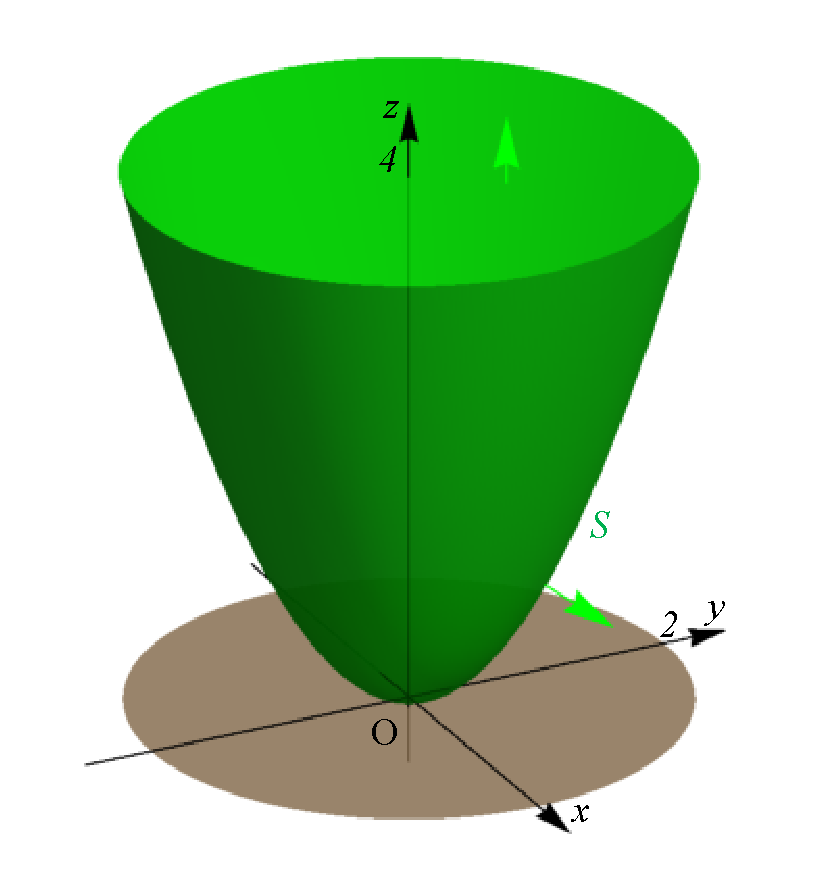
\includegraphics[height=0.5\textheight]{Figures24/Fig13-5-1-1.pdf}
\end{center}
\caption{习题13.5 1.(1)题图示}
\label{13-5-1-1}
\end{figure}

(2)记$\Omega$为$S^-$围成的区域,

$\because x^2,y^2,z^2\in C^1(\Omega)$,

$\therefore\BSIInt S{x^2\md y\wedge\md z+y^2\md z\wedge\md x+z^2\md x\wedge\md y}=-\BSIInt{S^-}{x^2\md y\wedge\md z+y^2\md z\wedge\md x+z^2\md x\wedge\md y}\\
=-\varIIInt\Omega{(\pp{x^2}x+\pp{y^2}y+\pp{z^2}z)}xyz=-\varIIInt\Omega{(2x+2y+2z)}xyz=0$.

\begin{figure}[H]
\begin{center}
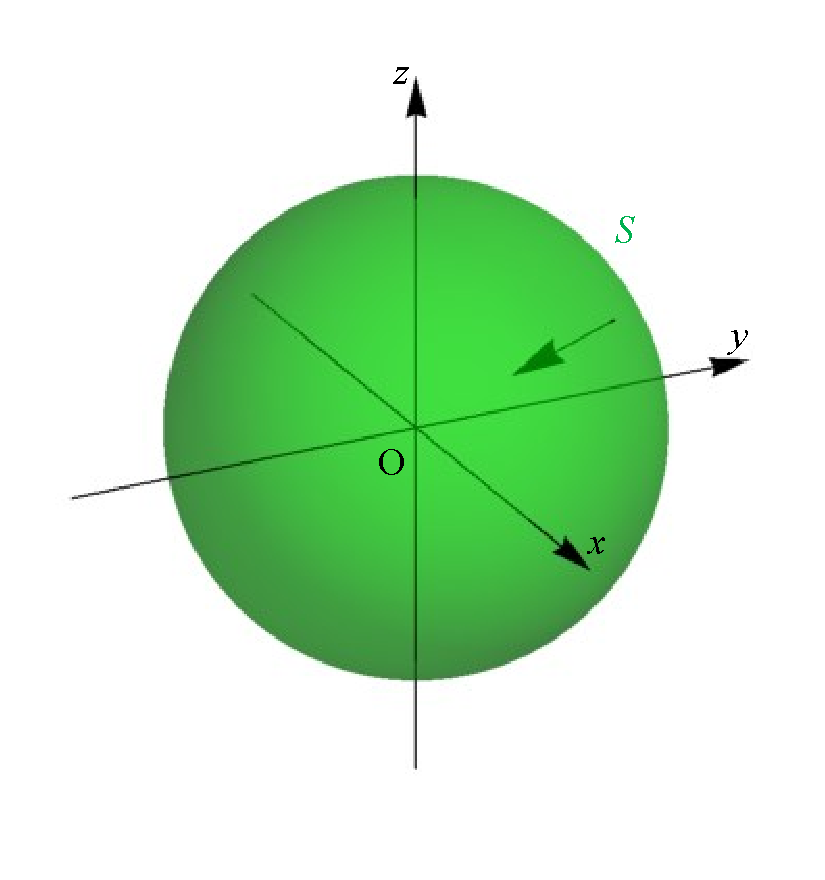
\includegraphics[height=0.5\textheight]{Figures24/Fig13-5-1-2.pdf}
\end{center}
\caption{习题13.5 1.(2)题图示}
\label{13-5-1-2}
\end{figure}

(3)$\because x^2,y^2,z^2\in C^1(\Omega)$,

$\therefore\BSIInt S{x^2\md y\wedge\md z+y^2\md z\wedge\md x+z^2\md x\wedge\md y}=\varIIInt\Omega{(\pp{x^2}x+\pp{y^2}y+\pp{z^2}z)}xyz\\
=2\varIIInt\Omega{(x+y+z)}xyz=6\varIIInt\Omega xxyz=6\Int01xx\Int01{}y\Int01{}z=6\Int01xx\Int01{}y\\
=6\Int01xx=3x^2\big|_0^1=3$.

\begin{figure}[H]
\begin{center}
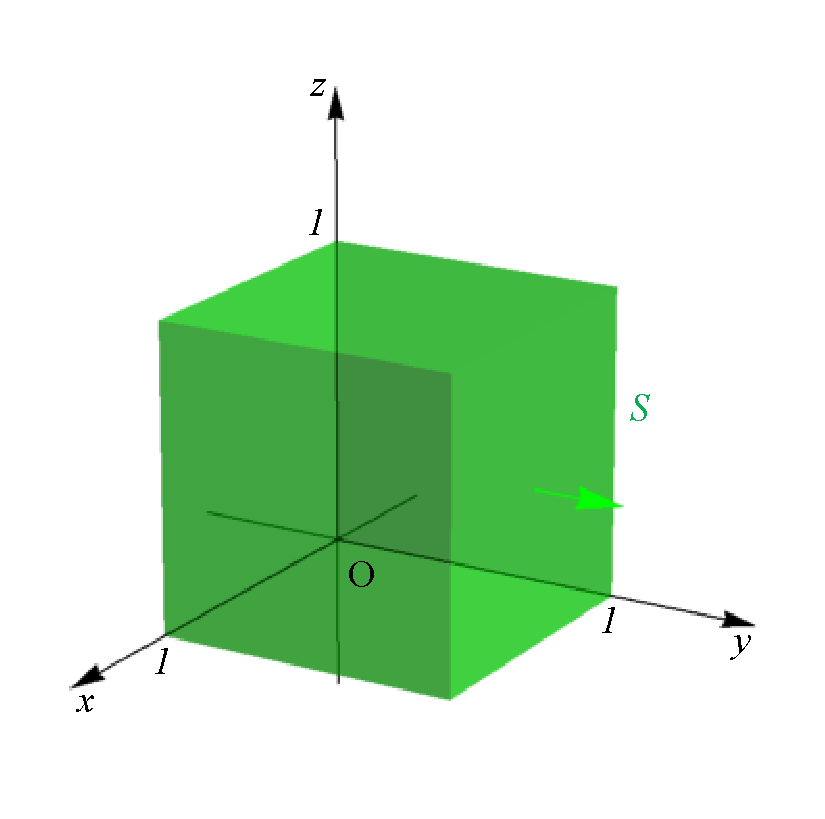
\includegraphics[height=0.5\textheight]{Figures24/Fig13-5-1-3.pdf}
\end{center}
\caption{习题13.5 1.(3)题图示}
\label{13-5-1-3}
\end{figure}

(4)记$S$围成的区域为$\Omega$,则$xz,xy,yz\in C^1(\Omega)$,

$\therefore\BSIInt S{xz\md x\wedge\md z+xy\md y\wedge\md z+yz\md z\wedge\md x}=\varIIInt\Omega{(\pp{xy}x+\pp{yz}y+\pp{xz}z)}xyz=\varIIInt\Omega{(y+z+x)}xyz\\
=3\varIIInt\Omega xxyz=3\Int01xx\Int0{1-x}{}y\Int0{1-x-y}{}z=3\Int01xx\Int0{1-x}{(1-x-y)}y\\
=3\Int01{x(y-xy-\frac12y^2)\big|_0^{1-x}}x=3\Int01{x(1-x-\frac12y)y\big|_0^{1-x}}x\\
=3\Int01{x[1-x-\frac12(1-x)](1-x)}x=3\Int01{x\frac12(1-x)^2}x=\frac32\Int01{x(1-2x+x^2)}x\\
=\frac32\Int01{(x-2x^2+x^3)}x=\frac32(\frac12x^2-\frac23x^3+\frac14x^4)\big|_0^1=\frac32(\frac12-\frac23+\frac14)=\frac32(\frac34-\frac23)=\frac32\cdot\frac1{12}=\frac18$.

\begin{figure}[H]
\begin{center}
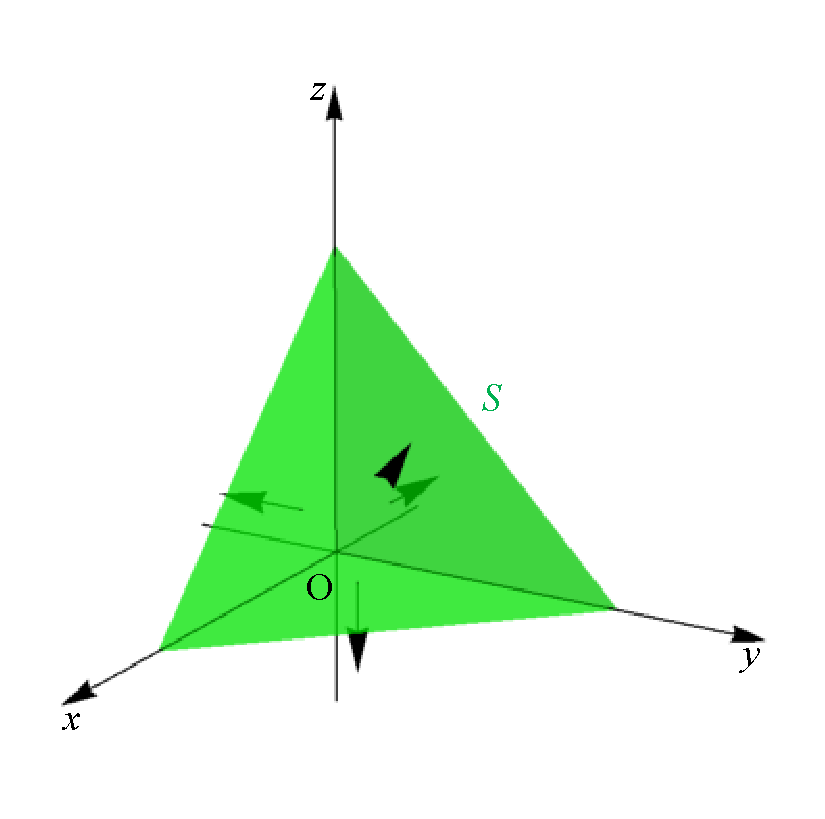
\includegraphics[height=0.5\textheight]{Figures24/Fig13-5-1-4.pdf}
\end{center}
\caption{习题13.5 1.(4)题图示}
\label{13-5-1-4}
\end{figure}

(5)取平面$S_1:z=1,x^2+y^2\leqslant1$,上侧为正,记$S$与$S_1$围成的区域为$\Omega$,

$\because x^2,z^2-2z\in C^1(\Omega)$,

$\therefore\BSIInt{S+S_1}{x^2\md y\wedge\md z+(z^2-2z)\md x\wedge\md y}=\varIIInt\Omega{(\pp{x^2}x+\pp0y+\pp{(z^2-2z)}z)}xyz\\
=\varIIInt\Omega{(2x+2z-2)}xyz$,

由对称性可知$\varIIInt\Omega{2x}xyz=0$,

$\therefore$上式$=\varIIInt\Omega{(2z-2)}xyz=\Int01{(2z-2)}z\varIInt{x^2+y^2\leqslant z^2}{}xy=\Int01{(2z-2)\pi z^2}z\\
=2\pi\Int01{(z^3-z^2)}z=2\pi(\frac14z^4-\frac13z^3)\big|_0^1=-\frac16\pi$,

$\because$在$S_1$上$\md\bm S=(-\pp zx,-\pp zy,1)\md x\md y=(0,0,1)\md x\md y=(\md y\wedge\md z,\md z\wedge\md x,\md x\wedge\md y)$,

$\therefore\BSIInt{S_1}{x^2\md y\wedge\md z+(z^2-2z)\md x\wedge\md y}=\varIInt{x^2+y^2\leqslant1}{[x^2\cdot0+(1^2-2\cdot1)]}xy=-\varIInt{x^2+y^2\leqslant1}{}xy=-\pi$,

$\therefore\BSIInt S{x^2\md y\wedge\md z+(z^2-2z)\md x\wedge\md y}=-\frac\pi6-\BSIInt{S_1}{x^2\md y\wedge\md z+(z^2-2z)\md x\wedge\md y}=-\frac\pi6+\pi=\frac56\pi$.

\begin{figure}[H]
\begin{center}
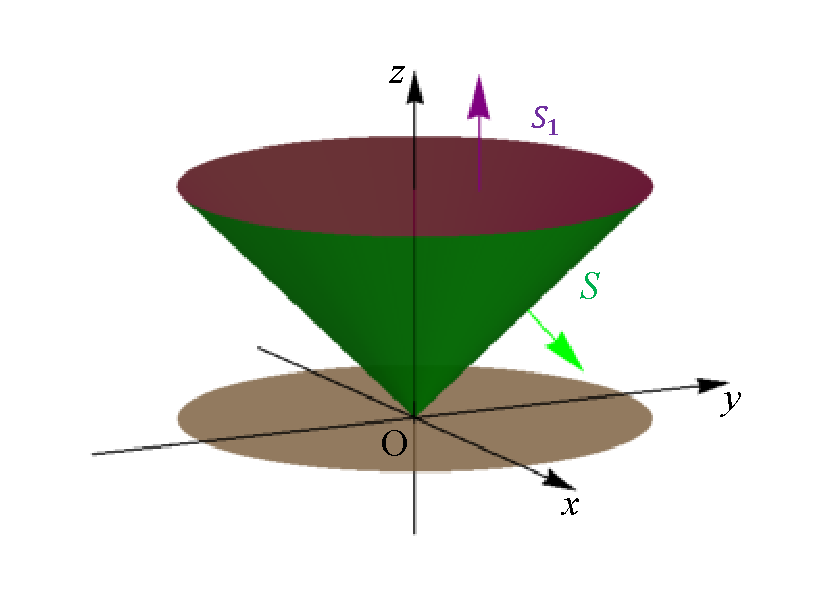
\includegraphics[height=0.5\textheight]{Figures24/Fig13-5-1-5.pdf}
\end{center}
\caption{习题13.5 1.(5)题图示}
\label{13-5-1-5}
\end{figure}

(6)记$S$围成的圆柱体区域为$\Omega$,则$x-y,(y-z)x\in C^1(\Omega)$,

$\therefore\BSOIInt S{(x-y)\md x\wedge\md y+(y-z)x\md y\wedge\md z}=\varIIInt\Omega{[\pp{(y-z)x}x+\pp0y+\pp{(x-y)}z]}xyz\\
=\varIIInt\Omega{(y-z)}xyz$,

由对称性可知$\varIIInt\Omega{y}xyz=0$,

$\therefore$上式$=-\varIIInt\Omega{z}xyz=-\Int13zz\varIInt{x^2+y^2\leqslant1}{}xy=-\pi\Int13zz=-\frac12\pi z^2\big|_1^3=-4\pi$.

\begin{figure}[H]
\begin{center}
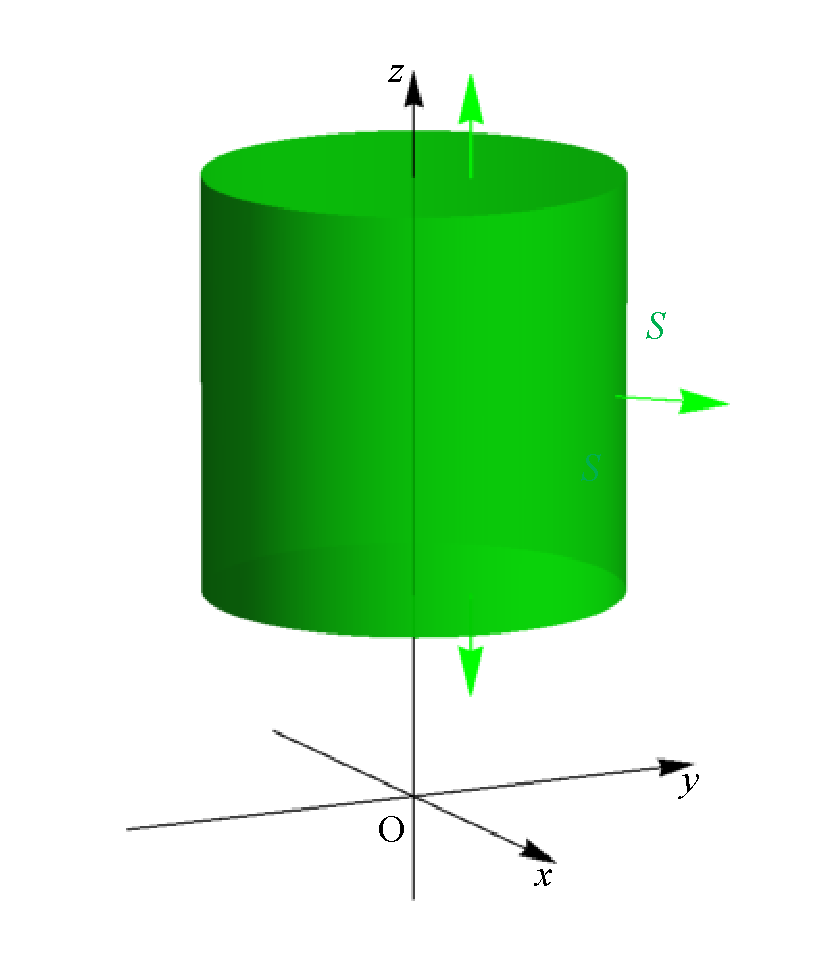
\includegraphics[height=0.5\textheight]{Figures24/Fig13-5-1-6.pdf}
\end{center}
\caption{习题13.5 1.(6)题图示}
\label{13-5-1-6}
\end{figure}

(7)取球面$S_1:\ x^2+y^2+z^2=r^2,r<\min\{a,b,c\}$,外侧为正,设$S$与$S_1^-$围成的区域为$\Omega$,$S_1$围成的区域为$\Omega_1$,

则$X=\frac x{(x^2+y^2+z^2)^{\frac32}},\ Y=\frac y{(x^2+y^2+z^2)^{\frac32}},\ Z=\frac z{(x^2+y^2+z^2)^{\frac32}}\in C^1(\Omega)$,
\[\begin{aligned}
\pp Xx=\frac{(x^2+y^2+z^2)^{\frac32}-x\cdot\frac32(x^2+y^2+z^2)^{\frac12}\cdot2x}{(x^2+y^2+z^2)^3}=\frac{y^2+z^2-2x^2}{(x^2+y^2+z^2)^{\frac52}},\\
\pp Yy=\frac{(x^2+y^2+z^2)^{\frac32}-y\cdot\frac32(x^2+y^2+z^2)^{\frac12}\cdot2y}{(x^2+y^2+z^2)^3}=\frac{z^2+x^2-2y^2}{(x^2+y^2+z^2)^{\frac52}},\\
\pp Zz=\frac{(x^2+y^2+z^2)^{\frac32}-z\cdot\frac32(x^2+y^2+z^2)^{\frac12}\cdot2z}{(x^2+y^2+z^2)^3}=\frac{x^2+y^2-2z^2}{(x^2+y^2+z^2)^{\frac52}},
\end{aligned}\]

$\therefore$
\[\begin{aligned}
&\BSOIInt{S+S_1^-}{\pp Xx\md y\wedge\md z+\pp Yy\md z\wedge\md x+\pp Zz\md x\wedge\md y}=\varIIInt\Omega{(\pp Xx+\pp Yy+\pp Zz)}xyz\\
=&\varIIInt\Omega{\frac{y^2+z^2-2x^2+z^2+x^2-2y^2+x^2+y^2-2z^2}{(x^2+y^2+z^2)^{\frac52}}}xyz=\varIIInt\Omega{0}xyz=0,
\end{aligned}\]
$\therefore$
\[\begin{aligned}
&\BSOIInt S{\frac{x\md y\wedge\md z+y\md z\wedge\md x+z\md x\wedge\md y}{(x^2+y^2+z^2)^{\frac32}}}=0-\BSOIInt{S_1^-}{\frac{x\md y\wedge\md z+y\md z\wedge\md x+z\md x\wedge\md y}{(x^2+y^2+z^2)^{\frac32}}}\\
=&\BSOIInt{S_1}{\frac{x\md y\wedge\md z+y\md z\wedge\md x+z\md x\wedge\md y}{(x^2+y^2+z^2)^{\frac32}}}=\BSOIInt{S_1}{\frac{x\md y\wedge\md z+y\md z\wedge\md x+z\md x\wedge\md y}{(r^2)^{\frac32}}}\\=&\frac1{r^3}\BSOIInt{S_1}{x\md y\wedge\md z+y\md z\wedge\md x+z\md x\wedge\md y}=\frac1{r^3}\varIIInt\Omega{(\pp xx+\pp yy+\pp zz)}xyz\\
=&\frac3{r^3}\varIIInt\Omega{}xyz=\frac3{r^3}\frac43\pi r^3=4\pi.
\end{aligned}\]
\begin{figure}[H]
\begin{center}
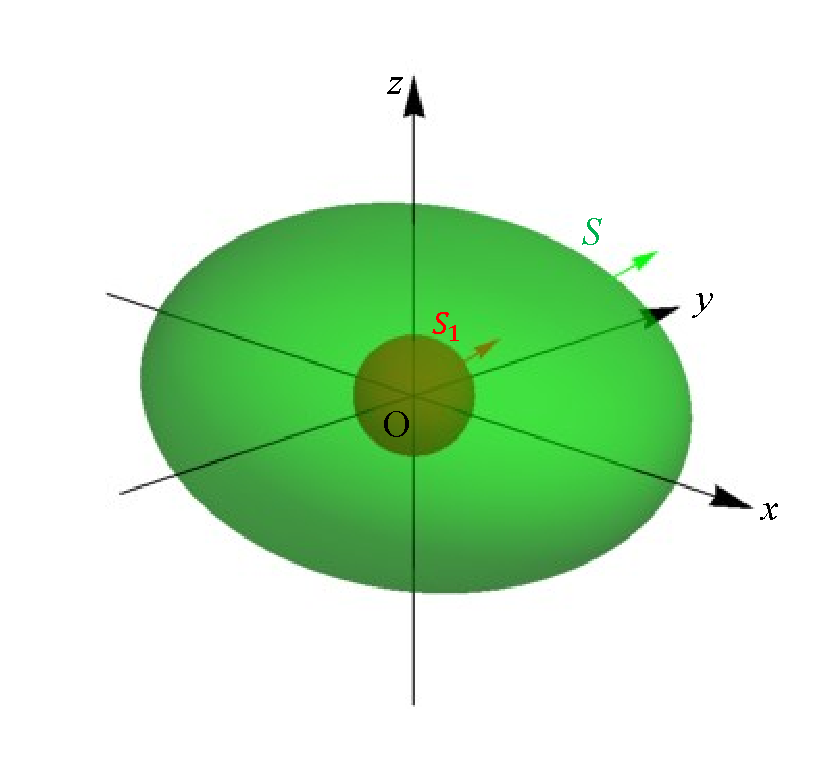
\includegraphics[height=0.5\textheight]{Figures24/Fig13-5-1-7.pdf}
\end{center}
\caption{习题13.5 1.(7)题图示}
\label{13-5-1-7}
\end{figure}
\item用斯托克斯公式计算下列曲线积分:\\
(1)$\BLOInt L{y\md x+z\md y+x\md z}$,其中$L$是圆周$\begin{cases}
x^2+y^2+z^2=R^2,\\
x+y+z=0,
\end{cases}$从$x$轴正向看去为逆时针方向;\\
(2)$\BLOInt L{(y-x)\md x+(z-y)\md y+(x-z)\md z}$,其中$L$是柱面$x^2+y^2=a^2$与平面$x+z=a(a>0)$的交线,从$x$轴正向看去为逆时针方向.

解:(1)记$\Sigma$是平面$x+y+z=0$上$L$围成的部分,$\Sigma$与$L$的方向符合右手法则,记$\Sigma$的上侧为正,

$\because y,z,x\in C^1$,

$\therefore\BLOInt L{y\md x+z\md y+x\md z}=\BSIInt\Sigma{\begin{vmatrix}
\bm i&\bm j&\bm k\\
\frac\partial{\partial x}&\frac\partial{\partial y}&\frac\partial{\partial z}\\
y&z&x
\end{vmatrix}\bm\cdot\bm n\md S}=\BSIInt\Sigma{(\pp xy-\pp zz,\pp zy-\pp xx,\pp zx-\pp yy)\bm\cdot\bm n\md S}\\
=\BSIInt\Sigma{(0-1,0-1,0-1)\bm\cdot\bm n\md S}=\BSIInt\Sigma{(-1,-1,-1)\bm\cdot\bm n\md S}$,

$\because\Sigma$的单位法向量为$\bm n=(1,1,1)\frac1{\sqrt3}$,

$\therefore\BLOInt L{y\md x+z\md y+x\md z}=\BSIInt\Sigma{(-1,-1,-1)\bm\cdot(1,1,1)\frac1{\sqrt3}\md S}=\frac1{\sqrt3}\BSIInt\Sigma{-3\md S}=-\sqrt3\pi R^2$.

\begin{figure}[H]
\begin{center}
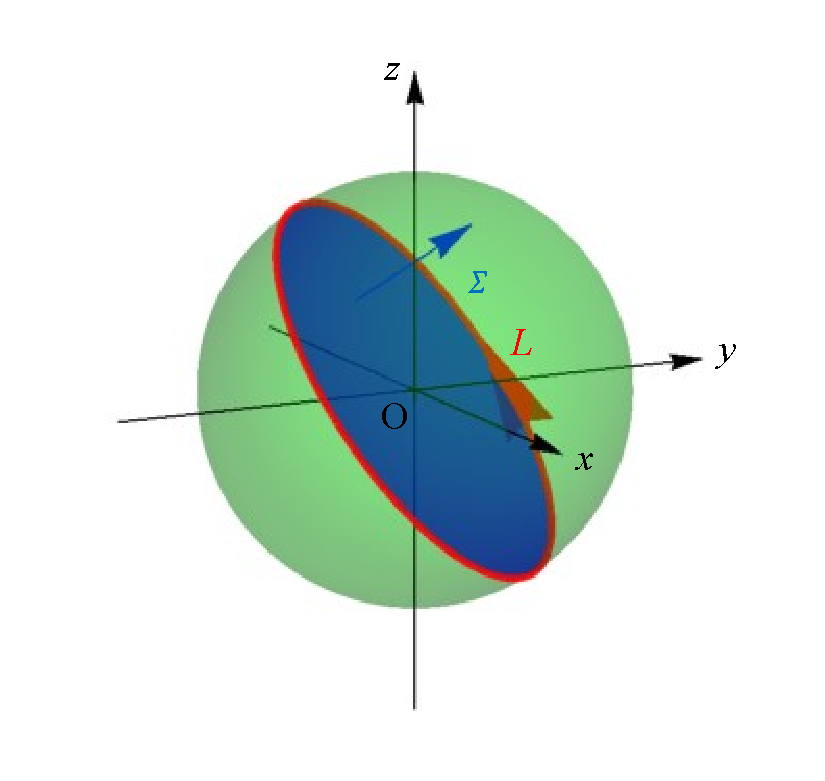
\includegraphics[height=0.5\textheight]{Figures24/Fig13-5-2-1.pdf}
\end{center}
\caption{习题13.5 2.(1)题图示}
\label{13-5-2-1}
\end{figure}

(2)记$\Sigma$是平面$x+z=a$上$L$围成的部分,$\Sigma$的方向与$L$的方向符合右手法则,即$\Sigma$的上侧为正,

$\because y-x,z-y,x-z\in C^1$,

$\therefore\BLOInt L{(y-x)\md x+(z-y)\md y+(x-z)\md z}=\BSIInt\Sigma{\begin{vmatrix}
\bm i&\bm j&\bm k\\
\frac\partial{\partial x}&\frac\partial{\partial y}&\frac\partial{\partial z}\\
y-x&z-y&x-z
\end{vmatrix}\bm\cdot\md\bm S}\\
=\BSIInt\Sigma{(\pp{(x-z)}y-\pp{(z-y)}z,\pp{(y-x)}z-\pp{(x-z)}x,\pp{(z-y)}x-\pp{(y-x)}y)\bm\cdot\md\bm S}=\BSIInt\Sigma{(0-1,0-1,0-1)\bm\cdot\md\bm S}$,

$\because$在$\Sigma:z=a-x,x^2+y^2\leqslant a^2$的上侧\\
$\md\bm S=(-\pp zx,-\pp zy,1)\md x\md y=(1,0,1)\md x\md y=(\md y\wedge\md z,\md z\wedge\md x,\md x\wedge\md y)$,

$\therefore$上式$=\varIInt{x^2+y^2\leqslant a^2}{(0-1,0-1,0-1)\bm\cdot(1,0,1)}xy=-2\varIInt{x^2+y^2\leqslant a^2}{}xy=-2\pi a^2$.

\begin{figure}[H]
\begin{center}
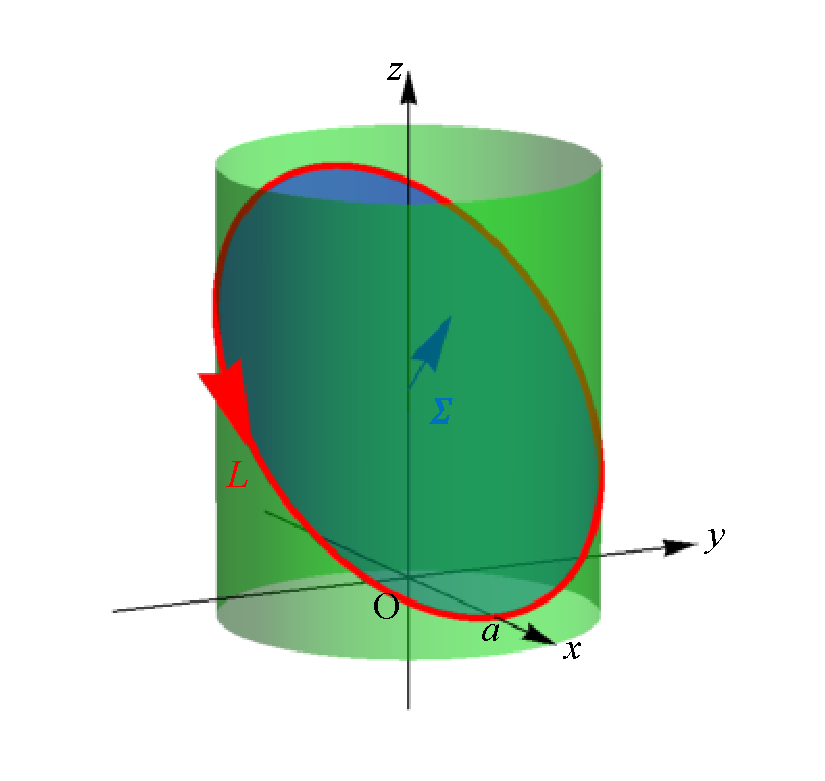
\includegraphics[height=0.5\textheight]{Figures24/Fig13-5-2-2.pdf}
\end{center}
\caption{习题13.5 2.(2)题图示}
\label{13-5-2-2}
\end{figure}
\item计算$I=\BLOInt L{\frac{-y\md x+x\md y}{x^2+y^2}+z\md z}$,其中$L$是:\\
(1)任意一条既不环绕$z$轴,也不与$z$轴相交的简单闭曲线;\\
(2)任意一条环绕$z$轴一圈且不与$z$轴相交的简单闭曲线,从$z$轴正向看去为逆时针方向.

解:(1)取曲面$\Sigma$为曲线$L$围成的逐片光滑有向曲面,$\Sigma$和$L$的方向符合右手法则,$z$轴不穿过$\Sigma$,

则$X=\frac{-y}{x^2+y^2},\ Y=\frac x{x^2+y^2},\ Z=z\in C^1$,

$\therefore$
\[\begin{aligned}
I&=\BLOInt L{X\md x+Y\md y+Z\md z}=\BSIInt\Sigma{\begin{vmatrix}
\bm i&\bm j&\bm k\\
\frac\partial{\partial x}&\frac\partial{\partial y}&\frac\partial{\partial z}\\
X&Y&Z
\end{vmatrix}}\bm\cdot\md\bm S=\BSIInt\Sigma{\begin{vmatrix}
\bm i&\bm j&\bm k\\
\frac\partial{\partial x}&\frac\partial{\partial y}&\frac\partial{\partial z}\\
\frac{-y}{x^2+y^2}&\frac x{x^2+y^2}&z
\end{vmatrix}}\bm\cdot\md\bm S\\
&=\BSIInt\Sigma{(\frac{\partial z}{\partial y}-\frac\partial{\partial z}\frac x{x^2+y^2},\frac\partial{\partial z}\frac{-y}{x^2+y^2}-\frac{\partial z}{\partial x},\frac\partial{\partial x}\frac x{x^2+y^2}-\frac\partial{\partial y}\frac{-y}{x^2+y^2})\bm\cdot\md\bm S}\\
&=\BSIInt\Sigma{(0-0,0-0,\frac{(x^2+y^2)-x\cdot2x}{(x^2+y^2)^2}-\frac{-(x^2+y^2)+y\cdot2y}{(x^2+y^2)^2})\bm\cdot\md\bm S}\\
&=\BSIInt\Sigma{(0,0,0)\bm\cdot\md\bm S}=0.
\end{aligned}\]
\begin{figure}[H]
\begin{center}
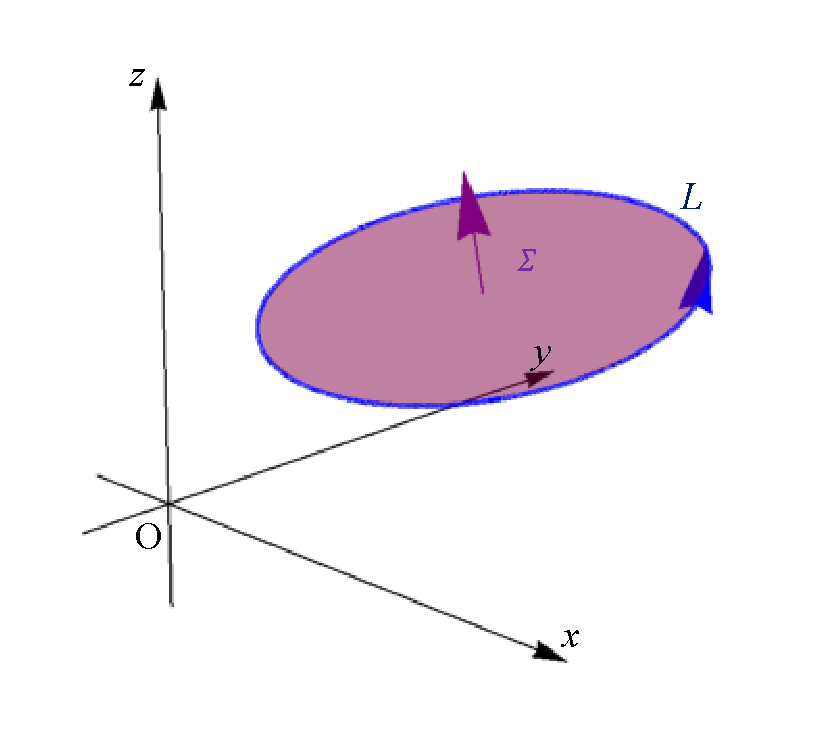
\includegraphics[height=0.5\textheight]{Figures24/Fig13-5-3-1.pdf}
\end{center}
\caption{习题13.5 3.(1)题图示}
\label{13-5-3-1}
\end{figure}

(2)设曲面$\Sigma$为曲线$L$围成的逐片光滑有向曲面,$\Sigma$与$L$的方向符合右手法则,即$\Sigma$的上侧为正,此时$z$轴穿过$\Sigma$. 取柱面$x^2+y^2=r^2$与$\Sigma$交于曲线$L_1$,$r$应足够小使得闭合交线$L_1$全部位于$\Sigma$上,设从$z$轴正向看去$L_1$为逆时针方向. 记$\Sigma_1$为$L_1$围成的逐片光滑正向曲面,$\Sigma_2$为$L$与$L_1^-$围成的逐片光滑正向曲面, $\Omega_2=\mathbb R^3\backslash\{(x,y)|x^2+y^2<r^2\}$.

则$X=\frac{-y}{x^2+y^2},\ Y=\frac x{x^2+y^2},\ Z=z\in C^1(\Omega_2)$,

与(1)同理可知$\BLOInt{L+L_1^-}{X\md x+Y\md y+Z\md z}=0$,

$\therefore$
\[\begin{aligned}
I&=0-\BLOInt{L_1^-}{X\md x+Y\md y+Z\md z}=\BLOInt{L_1}{X\md x+Y\md y+Z\md z}\\
&=\BLOInt{L_1}{\frac{-y\md x+x\md y}{x^2+y^2}+z\md z}=\BLOInt{L_1}{\frac{-y\md x+x\md y}{r^2}+z\md z}\\
&=\BSIInt{\Sigma_1}{\begin{vmatrix}
\bm i&\bm j&\bm k\\
\frac\partial{\partial x}&\frac\partial{\partial y}&\frac\partial{\partial z}\\
-\frac y{r^2}&\frac x{r^2}&z
\end{vmatrix}\bm\cdot\md\bm S}=\BSIInt{\Sigma_1}{(\pp zy-\frac\partial{\partial z}\frac x{r^2},\frac\partial{\partial z}(-\frac y{r^2})-\pp zx,\frac\partial{\partial x}\frac x{r^2}-\frac\partial{\partial y}(-\frac y{r^2}))\bm\cdot\md\bm S}\\
&=\BSIInt{\Sigma_1}{(0-0,0-0,\frac 1{r^2}-(-\frac 1{r^2}))\bm\cdot\md\bm S}=\BSIInt{\Sigma_1}{(0,0,\frac 2{r^2})\bm\cdot(\md y\wedge\md z,\md z\wedge\md x,\md x\wedge\md y)}\\
&=\BSIInt{\Sigma_1}{\frac 2{r^2}\md x\wedge\md y}=\frac 2{r^2}\BSIInt{\Sigma_1}{\md x\wedge\md y},
\end{aligned}\]
$\because\Sigma_1$方程可表示为$z=f(x,y),x^2+y^2\leqslant r^2$,且$\Sigma_1$上侧为正,

$\therefore I=\frac 2{r^2}\BSIInt{\Sigma_1}{\md x\wedge\md y}=\frac2{r^2}\varIInt{x^2+y^2\leqslant r^2}{}xy=\frac2{r^2}\pi r^2=2\pi$.
\begin{figure}[H]
\begin{center}
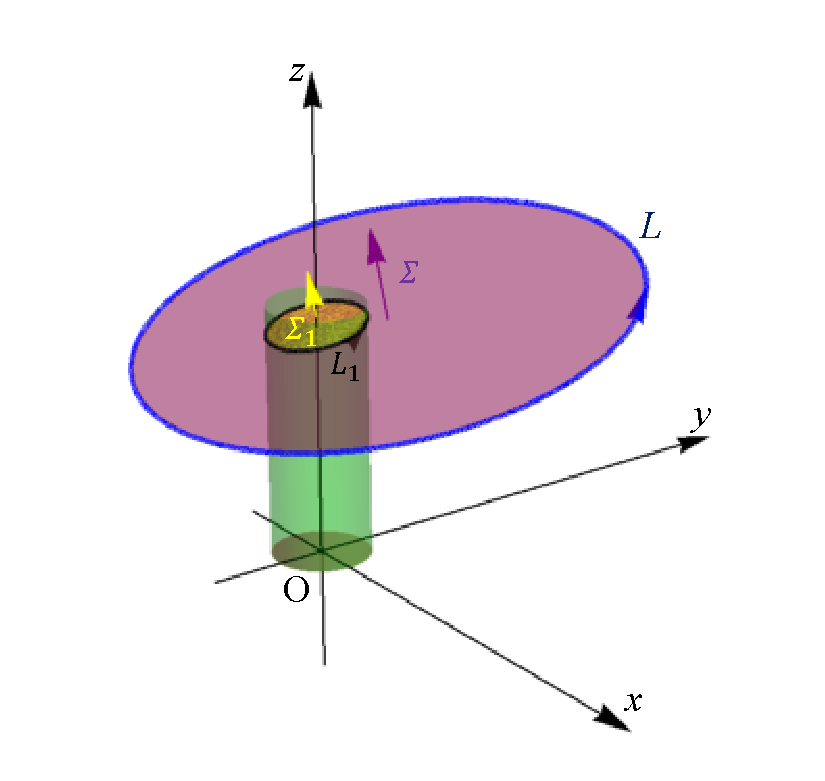
\includegraphics[height=0.7\textheight]{Figures24/Fig13-5-3-2.pdf}
\end{center}
\caption{习题13.5 3.(2)题图示}
\label{13-5-3-2}
\end{figure}
\item证明:
\[
\BLOInt L{\begin{vmatrix}
\md x&\md y&\md z\\
\cos\alpha&\cos\beta&\cos\gamma\\
x&y&z
\end{vmatrix}}=2S,
\]
其中$L$是$\mathbb R^3$中某个平面上的一条简单逐段光滑闭曲线,$\bm n=(\cos\alpha,\cos\beta,\cos\gamma)$是该平面的单位法向量,$L$的方向与$\bm n$的方向服从右手法则,$S$是$L$所围的面积.

证明:\[
\BLOInt L{\begin{vmatrix}
\md x&\md y&\md z\\
\cos\alpha&\cos\beta&\cos\gamma\\
x&y&z
\end{vmatrix}}=\BLOInt L{(z\cos\beta-y\cos\gamma)\md x+(x\cos\gamma-z\cos\alpha)\md y+(y\cos\alpha-x\cos\beta)\md z},
\]


记$\Sigma$是$L$在该平面上围成的部分,$\Sigma$的方向与$\bm n$的方向一致,则$\Sigma$的面积为$S$,$z\cos\beta-y\cos\gamma,x\cos\gamma-z\cos\alpha,y\cos\alpha-x\cos\beta\in C^1(\Sigma)$,

$\therefore$
\[\begin{aligned}
\text{上式}&=\BSIInt\Sigma{\begin{vmatrix}
\bm i&\bm j&\bm k\\
\frac\partial{\partial x}&\frac\partial{\partial y}&\frac\partial{\partial z}\\
z\cos\beta-y\cos\gamma&x\cos\gamma-z\cos\alpha&y\cos\alpha-x\cos\beta
\end{vmatrix}}\\
&=\BSIInt\Sigma{\{[\pp{(y\cos\alpha-x\cos\beta)}x-\pp{(x\cos\gamma-z\cos\alpha)}z]\bm i\\
&\hspace{3cm}+[\pp{(z\cos\beta-y\cos\gamma)}z-\pp{(y\cos\alpha-x\cos\beta)}x]\bm j\\
&\hspace{5cm}+[\pp{(x\cos\beta-z\cos\alpha)}x-\pp{(z\cos\beta-y\cos\gamma)}y]\bm k\}\bm\cdot\bm n\md S}\\
&=\BSIInt\Sigma{\{[\cos\alpha-(-\cos\alpha)]\bm i+[\cos\beta-(-\cos\beta)]\bm j+[\cos\gamma-(-\cos\gamma)]\bm k\}\bm\cdot\bm n\md S}\\
&=\BSIInt\Sigma{(2\cos\alpha\bm i+2\cos\beta\bm j+2\cos\gamma\bm k)\bm\cdot\bm n\md S}\\
&=\BSIInt\Sigma{(2\cos\alpha,2\cos\beta,2\cos\gamma)\bm\cdot(\cos\alpha,\cos\beta,\cos\gamma)\md S}\\
&=\BSIInt\Sigma{(2\cos^2\alpha+2\cos^2\beta+2\cos^2\gamma)\md S}\\
&=2\BSIInt\Sigma{\md S}=2S.
\end{aligned}\]
\end{enumerate}
\end{document}